\section{Gradient Descent on Logistic Regression}

\begin{enumerate}
    \item Accuracy on the test set:  0.77
    
    Logistic regression coefficient(Scikit):
    [ 1.30299939e-04  1.76132834e-06 -1.30923960e-06 -3.08981964e-04
  -3.31896546e-04  5.17574298e-04  6.98099943e-07 -3.10110604e-07
  -3.23366122e-07 -3.70267292e-04 -1.84436862e-07]
    \item 
    Log Likelihood:
    $$
    -LL = -\frac{1}{N} \sum_{n = 1}^{N}y_n(log(h_w(x_n))) + (1-y_n) (log(1-h_w(x_n)))
    $$
    
    Derivative:
    $$
    dw = \frac{1}{N}\sum_{n = 1}^{N}(h_w(x_n)-y_n)x_n 
    $$
    
    Update formula:
    $$
    w = w-\frac{\eta}{N}\sum_{n = 1}^{N}(h_w(x_n)-y_n)x_n
    $$ 
    $\eta$: learning rate; N: the size of training data.
    \item Accuracy on the training set: 0.76375
    
    Accuracy on the test set: 0.7675
    
    Logistic regression coefficient (SGD):
    [ 5.67051726e-03  5.21208621e-02 -1.10211910e-02 -2.57983118e-01
  -9.05115041e-01  3.51256199e+00  1.55306123e-02 -1.54856541e-02
  -6.68514118e-03 -1.74995599e+00 -8.72165559e-04]
  
    \item Accuracy on the training set: 0.82375
    
    Accuracy on the test set: 0.815
    
    Logistic regression coefficient (AdaGrad):
    [ 8.56662029e-05  7.32614095e-03 -4.06503117e-03 -1.84270727e-04
  -1.05933198e-03  4.09573976e-03  7.04325651e-03 -7.02782768e-03
  -6.96842728e-03 -2.22061369e-03 -2.21480516e-03]
    \item 
    The AdaGrad algorithm has better accuracy on the training set. Because of the feature which is frequently learned, the learning rate of this feature is small. Because the sum of the gradient at each step is very large and the learning rate will be comparably large. Thus, the AdaGrad algorithm learn slowly but pay more attention to rare and informative feature.
    \begin{figure}[H]
    \caption{Accuracy vs. iteration for SGD and AdaGrad (2 points)}
        \centering            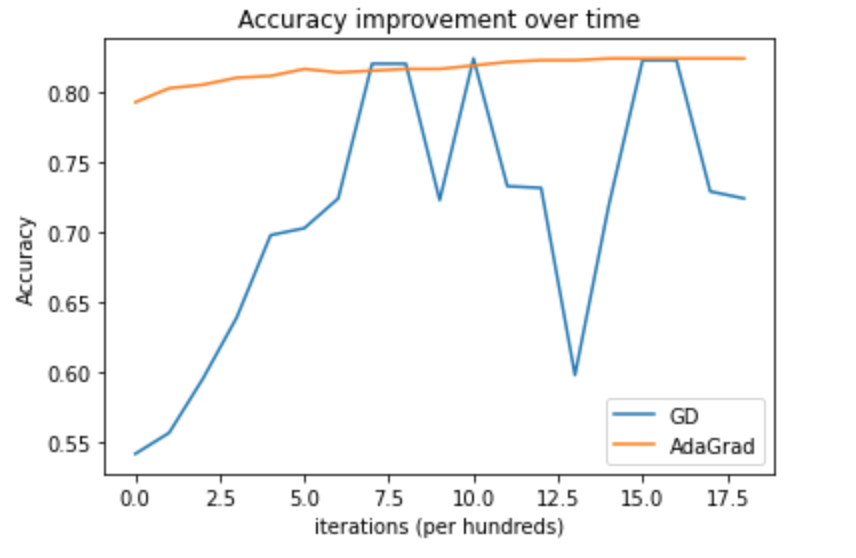
\includegraphics[width=0.5\textwidth]{images/8.png}
    \end{figure}
    
\end{enumerate}